\documentclass[12pt, a4paper]{article}

\usepackage[czech]{babel}
\usepackage{lmodern}
\usepackage[utf8]{inputenc}
\usepackage[T1]{fontenc}
\usepackage[pdftex]{graphicx}
\usepackage{amsmath, amssymb}
\usepackage[hidelinks,unicode]{hyperref}
\usepackage{float}
\usepackage{listings}
\usepackage{tikz}
\usepackage{xcolor}
\usepackage{tabularx}
\usepackage[final]{pdfpages}
\usepackage{syntax}
\usepackage{caption}
\usepackage{subcaption}
\usepackage{amsfonts}


\definecolor{mauve}{rgb}{0.58,0,0.82}
\usetikzlibrary{shapes,positioning,matrix,arrows}

\newcommand{\img}[1]{(viz obr. \ref{#1})}

\definecolor{pblue}{rgb}{0.13,0.13,1}
\definecolor{pgreen}{rgb}{0,0.5,0}
\definecolor{pred}{rgb}{0.9,0,0}
\definecolor{pgrey}{rgb}{0.46,0.45,0.48}


\lstdefinestyle{flex}{
    frame=tb,
    aboveskip=3mm,
    belowskip=3mm,
    showstringspaces=false,
    columns=flexible,
    basicstyle={\small\ttfamily},
    numbers=none,
    numberstyle=\tiny\color{black},
    keywordstyle=\color{black},
    commentstyle=\color{black},
    stringstyle=\color{black},
    breaklines=true,
    breakatwhitespace=true,
    tabsize=3
}

\lstset{
    frame=tb,
    language=Python,
    aboveskip=3mm,
    belowskip=3mm,
    showstringspaces=false,
    columns=flexible,
    basicstyle={\small\ttfamily},
    numbers=none,
    numberstyle=\tiny\color{gray},
    keywordstyle=\color{blue},
    commentstyle=\color{pgreen},
    stringstyle=\color{mauve},
    breaklines=true,
    breakatwhitespace=true,
    tabsize=3
}


\let\oldsection\section
\renewcommand\section{\clearpage\oldsection}

\begin{document}
	% this has to be placed here, after document has been created
	% \counterwithout{lstlisting}{chapter}
	\renewcommand{\lstlistingname}{Ukázka kódu}
	\renewcommand{\lstlistlistingname}{Seznam ukázek kódu}
    \begin{titlepage}

        \centering

        \vspace*{\baselineskip}
        \begin{figure}[H]
        \centering
        
\includegraphics[width=7cm]{img/fav-logo.jpg}
        \end{figure}

        \vspace*{1\baselineskip}

        \vspace{0.75\baselineskip}

        \vspace{0.5\baselineskip}
        {Domácí úkol z předmětu KIV/VSS}

        {\LARGE\sc Markovské náhodné procesy a systémy hromadné obsluhy\\}
        {\sc M/G/1\\}

        \vspace{4\baselineskip}

        \vspace{0.5\baselineskip}

        {\sc\Large Stanislav Král \\}
        \vspace{0.5\baselineskip}
        {A20N0091P}

        \vfill

        {\sc Západočeská univerzita v Plzni\\
        Fakulta aplikovaných věd}

    \end{titlepage}

    % TOC
    \tableofcontents
    \pagebreak

\section{Zadání}
Vytvořte markovský model obslužného systému M/G/1 s délkou fronty omezenou na 1. Vstupní proud má střední frekvenci lambda= 1.0. Obsluha se skládá ze dvou navazujících částí (fází), každá část má dobu trvání s exp. rozdělením s parametrem mi=2.0. Z modelu určete:
\begin{itemize}
    \item střední periodu, se kterou dochází k úplnému vyprázdnění systému (tj. stavu, kdy v systému není žádný požadavek),
    \item pravděpodobnost, že se v systému nachází právě jeden požadavek.
\end{itemize}

\section{Vypracování}

Graf popisující vytvořený markovský model dle zadání:

\begin{figure}[!ht]
    \centering
    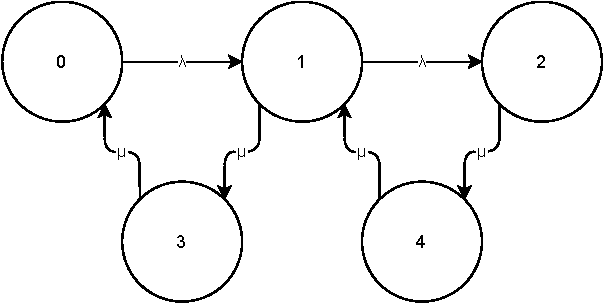
\includegraphics[width=.95\linewidth]{pdf/graph.pdf}
    \captionof{figure}{Graf vytvořeného markovského modelu}
    \label{fig:test1}
\end{figure}

\noindent Popis významu jednotlivých stavů:
\begin{itemize}
    \item \textbf{0} -- v systému není zpracováván žádný požadavek a fronta je prázdná
    \item \textbf{1} -- v systému je zpracováván jeden požadavek a fronta je prázdná
    \item \textbf{2} -- v systému je zpracováván jeden požadavek a ve frontě čeká na obsloužení jeden požadavek
    \item \textbf{3} -- v systému je zpracováván jeden požadavek, jehož první část obsluhy byla zpracována a fronta je prázdná
    \item \textbf{4} -- v systému je zpracováván jeden požadavek, jehož první část obsluhy byla zpracována a ve frontě čeká na obsloužení jeden požadavek
\end{itemize}

\noindent Popis významu přechodů mezi stavy:
\begin{itemize}
    \item $0 \rightarrow 1$ -- vstup požadavku do systému, který bude ihned zpracováván
    \item $1 \rightarrow 2$ -- vstup požadavku do systému, který bude umístěn do fronty
    \item $1 \rightarrow 3$ -- dokončení první části zpracovávání požadavku v systému
    \item $2 \rightarrow 4$ -- dokončení první části zpracovávání požadavku v systému
    \item $3 \rightarrow 0$ -- dokončení druhé části zpracovávání požadavku v systému, které vede k odebrání požadavku ze systému
    \item $4 \rightarrow 1$ -- dokončení druhé části zpracovávání požadavku v systému, které vede k odebrání požadavku ze systému
\end{itemize}

\noindent Popis modelu Kolmogorovovy rovnicemi je následující:
\begin{equation}
    \begin{split}
    & p'_{0}(t) = \mu p_{3}(t) - \lambda p_{0}(t) \\
    & p'_{1}(t) = \lambda p_{0}(t) + \mu p_{4}(t) - \lambda p_{1}(t) - \mu p_{3}(t) \\
    & p'_{2}(t) = \lambda p_{1}(t) - \mu p_{2}(t) \\
    & p'_{3}(t) = \mu p_{1}(t) - \mu p_{3}(t) \\
    & p'_{4}(t) = \mu p_{2}(t) - \mu p_{4}(t) \\
    \end{split}
\end{equation}

Postup sestavení soustavy s limitními pravděpodobnostmi a normalizační rovnicí za účelem vyjádření pravděpodobností setrvávání v jednotlivých stavech je následující:

\begin{equation}
    \begin{split}
    & 0 = \mu p_{3} - \lambda p_{0} \\
    & 0 = \lambda p_{1} - \mu p_{2} \\
    & 0 = \mu p_{1} - \mu p_{3} \\
    & 0 = \mu p_{2} - \mu p_{4} \\
    & 1 = p_{0} + p_{1} + p_{2} + p_{3} + p_{4}
    \\
    & p_{1} = \frac{\lambda}{\mu} p_0 \\
    & p_{2} = \frac{\lambda^2}{\mu^2} p_0 \\
    & p_{3} = \frac{\lambda}{\mu} p_0 \\
    & p_{4} = \frac{\lambda^2}{\mu^2} p_0 \\
    \\
    & 1 = p_{0} + \frac{\lambda}{\mu} p_0 + \frac{\lambda^2}{\mu^2} p_0 + \frac{\lambda}{\mu} p_0 + \frac{\lambda^2}{\mu^2} p_0 \\
    & p_{0} = \frac{\mu^2}{\mu^2 + 2\lambda\mu + 2\lambda^2} \\
    \end{split}
\end{equation}

\pagebreak
\noindent Po dosazení hodnot $\lambda=1$ a $\mu=2$ ze zadání dostáváme:

\begin{equation}
    \begin{split}
    & p_{0} = 0.4 \\
    & p_{1} = 0.2 \\
    & p_{2} = 0.1 \\
    & p_{3} = 0.2 \\
    & p_{4} = 0.1 \\
    \end{split}
\end{equation}

Výpočet středních period přechodů mezi hranami $1 \rightarrow 3$ a $3 \rightarrow 0$ je následující:

\begin{equation}
    \begin{split}
    & f_{i, j} = p_{i} * \lambda_{i, j} \\
    & f_{1, 3} = p_{1} * \lambda_{1, 3} = 0.2 * 2 = 0.4 \\
    & f_{3, 0} = p_{3} * \lambda_{3, 0} = 0.2 * 2 = 0.4 \\
    & \\
    & T_{1, 3} = \frac{1}{f_{1, 3}} = 2.5 \\
    & T_{3, 0} = \frac{1}{f_{3, 0}} = 2.5 \\
    \end{split}
\end{equation}

Střední periodu, se kterou dochází k úplnému vyprázdnění systému, lze vypočítat tak, že sečteme střední periody přechodů mezi hranami $T_{1, 3}$ a $T_{3, 0}$\footnote{Nejsem si zcela jistý, zdali je toto tvrzení pravdivé a výpočet požadované periody správný.}.

\begin{equation}
    \begin{split}
    & T_{vypr} = T_{1, 3} + T_{3, 0} = 2.5 + 2.5 = 5 \\ 
    \end{split}
\end{equation}

Pravděpodobnost, že se v systému nachází právě jeden požadavek, lze vyjádřit jako součet pravděpodobností, že model setrvává ve stavech \textbf{1} a \textbf{3}, tedy když je zpracovávaná první nebo druhá část požadavku a fronta je prázdná.

\begin{equation}
    \begin{split}
    & p_{jeden} = p_{1} + p_{3} = 0.2 + 0.2 = 0.4 \\ 
    \end{split}
\end{equation}

\end{document}

